\documentclass[border=6pt]{standalone}
\usepackage[T1]{fontenc}
\usepackage{helvet}
\renewcommand\familydefault{\sfdefault}
\usepackage{tikz}
\usetikzlibrary{positioning,arrows.meta,shapes.geometric,calc,bending}

\hyphenation{arrow}

\begin{document}
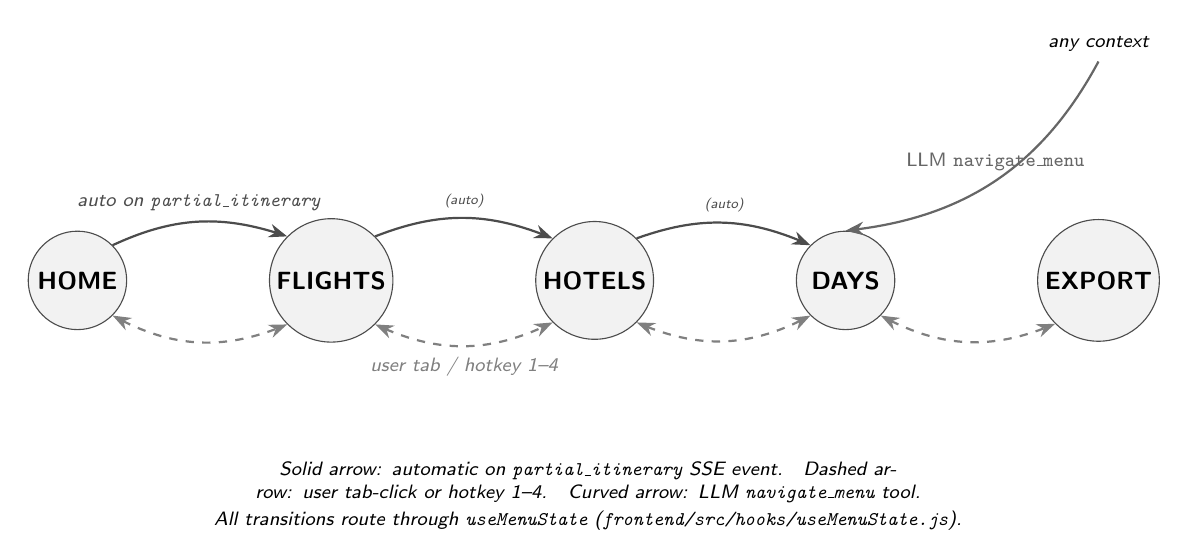
\begin{tikzpicture}[
  font=\small,
  >=Stealth,
  state/.style={circle, draw=black!70, fill=gray!10,
                minimum size=1.25cm, font=\small\bfseries,
                inner sep=2pt, align=center},
]

% Five panel nodes in a row
\node[state] (home)    {HOME};
\node[state, right=1.8cm of home]    (flights) {FLIGHTS};
\node[state, right=1.8cm of flights] (hotels)  {HOTELS};
\node[state, right=1.8cm of hotels]  (days)    {DAYS};
\node[state, right=1.8cm of days]    (export)  {EXPORT};

% --- Solid automatic arrows (SSE-driven) ---
% Label the first arrow only; the two unlabeled ones carry a small "(auto)" tag
\draw[->, thick, black!70]
  (home.north east) to[bend left=22]
  node[above, font=\scriptsize\itshape, midway]
    {auto on \texttt{partial\_itinerary}}
  (flights.north west);

\draw[->, thick, black!70]
  (flights.north east) to[bend left=22]
  node[above, font=\tiny\itshape, midway] {(auto)}
  (hotels.north west);

\draw[->, thick, black!70]
  (hotels.north east) to[bend left=22]
  node[above, font=\tiny\itshape, midway] {(auto)}
  (days.north west);

% --- Dashed bidirectional arrows (user tab / hotkey) ---
% Label the middle arrow only to avoid repetition
\draw[<->, thick, dashed, black!50]
  (home.south east) to[bend right=26] (flights.south west);

\draw[<->, thick, dashed, black!50]
  (flights.south east) to[bend right=26]
  node[below, font=\scriptsize\itshape, midway] {user tab / hotkey 1--4}
  (hotels.south west);

\draw[<->, thick, dashed, black!50]
  (hotels.south east) to[bend right=26] (days.south west);

\draw[<->, thick, dashed, black!50]
  (days.south east) to[bend right=26] (export.south west);

% --- Curved navigate_menu arrow: from upper-right (clear of auto labels) into days ---
\draw[->, thick, black!60]
  ($(export.north) + (0, 2.0)$)
  to[bend left=28]
  node[above, font=\scriptsize, midway]
    {LLM \texttt{navigate\_menu}}
  (days.north);

\node[font=\scriptsize\itshape, anchor=south] at ($(export.north) + (0, 2.0)$)
  {any context};

% --- Legend line below diagram ---
\node[font=\scriptsize, anchor=north, text width=13cm, align=center,
      inner sep=0pt]
  at ($(home.south)!0.5!(export.south) + (0,-1.6)$) {%
  \itshape
  Solid arrow: automatic on \texttt{partial\_itinerary} SSE event.\quad
  Dashed arrow: user tab-click or hotkey 1--4.\quad
  Curved arrow: LLM \texttt{navigate\_menu} tool.\\[2pt]
  All transitions route through
  \texttt{useMenuState} (\texttt{frontend/src/hooks/useMenuState.js}).%
};

\end{tikzpicture}
\end{document}
